\subsection{Режим имитовставки}\index{имитовствка!(}
\selectlanguage{russian}

Режим выработки имитовставки (рис.~\ref{fig:GOST_MAC}, \cite{GOST-89}) принципиально отличается от рассмотренных ранее режимов тем, что призван обеспечивать не конфиденциальность, а целостность. Результатом является блок данных фиксированного размера (в ГОСТ 28147-89 -- до 32 бит), длина которого не зависит от длины исходного сообщения.

\begin{figure}[bt]
	\centering
	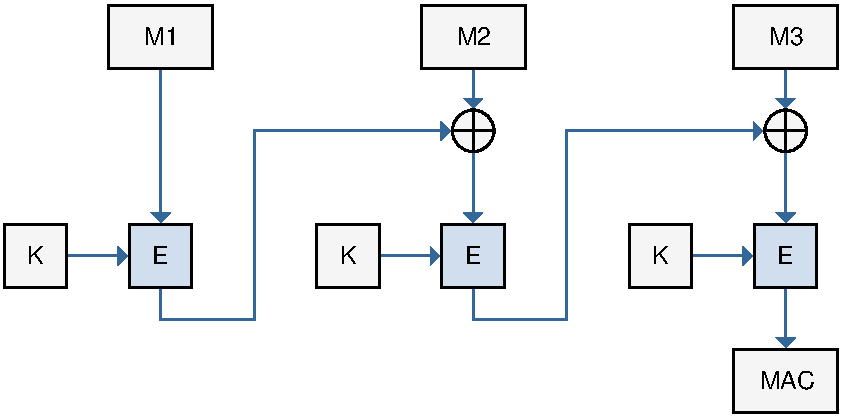
\includegraphics[width=1\textwidth]{pic/GOST_MAC}
	\caption{Режим выработки имитовставки}
	\label{fig:GOST_MAC}
\end{figure}

Входное сообщение как и ранее разбивается на блоки равной длины $M_1, M_2, \dots, M_n$. Последний блок, при необходимости, дополняется (ГОСТ 28147-89 -- нулями). Формула выработки имитовставки выглядит следующим образом:

\[ \begin{array}{l}
	X_1 = M_1; \\
	Y_j = E_K ( X_j ), ~ j = 1, 2, \dots, n; \\
	X_j = Y_{j-1} \oplus M_j, ~ j = 2, \dots, n; \\
	\textbf{MAC} = Y_n.
\end{array} \]

В ГОСТ 28147-89 для режима выработки имитовставки функция шифрования использует 16 раундов вместо 32.

Как уже было сказано, данный режим обеспечивает только целостность информации. Причём саму информацию необходимо передавать, и, возможно, шифровать отдельно. Режим не обеспечивает возможности параллельных вычислений для разных блоков открытого текста.

Принципиальным недостатком является необходимость использовать секретный ключ\index{ключ!секретный} как для выработки имитовставки, так и для её валидации (путём повторной выработки на принимающей стороне и сравнения с результатом). Позже мы рассмотрим функциональных электронных цифровых подписей, которые по своему назначению схожи с имитовставкой, но обеспечивают вариант более гибкого использования -- без необходимости раскрытия ключа, используемого для генерации ЭЦП.

\index{имитовствка!)}